\tikzstyle{vertex}=[circle,fill=black!15,minimum size=20pt,inner sep=0pt]
\tikzstyle{job vertex} = [vertex, fill=red!50]
\tikzstyle{completed vertex} = [vertex, fill=red!24]
\tikzstyle{possible vertex} = [vertex, fill=black!25]
\tikzstyle{edge} = [draw,thick,->,black!20]
\tikzstyle{proc} = [font=\small, below]
\tikzstyle{completed edge} = [draw,line width=2pt,->,red!50]
\tikzstyle{possible edge} = [draw,line width=4pt,->,black!20]

\begin{figure}[p]\centering
    \subcaptionbox{$k=0$\label{fig:example:graph:empty}}{
    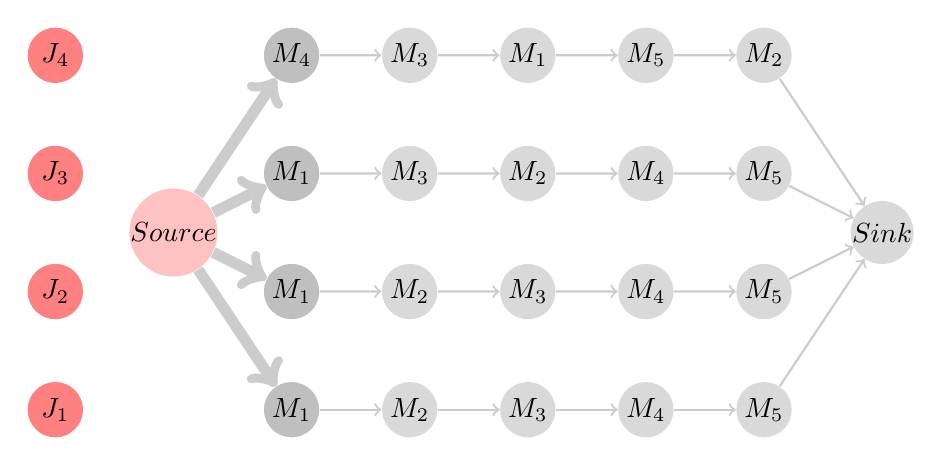
\begin{tikzpicture}[scale=1.5, auto, swap]
    % Draw the network
    % First we draw the jobs
    \foreach \pos/\name in {{(-1,0)/J_1},{(-1,1)/J_2},{(-1,2)/J_3},{(-1,3)/J_4}}
    \node[job vertex] (\name) at \pos {$\name$};    
    % Second draw the machines / vertices    
    \foreach \pos/\name/\mac/\proc in {{(0,1.5)/Source}}
    \node[completed vertex] (\name) at \pos {$\mac$};
    \foreach \pos/\name/\mac/\proc in {{(6,1.5)/Sink},
        {(2,0)/J1M2/M_2/25},{(3,0)/J1M3/M_3/40},{(4,0)/J1M4/M_4/15},{(5,0)/J1M5/M_5/42},
        {(2,1)/J2M2/M_2/86},{(3,1)/J2M3/M_3/86},{(4,1)/J2M4/M_4/68},{(5,1)/J2M5/M_5/84},
        {(2,2)/J3M3/M_3/23},{(3,2)/J3M2/M_2/59},{(4,2)/J3M4/M_4/33},{(5,2)/J3M5/M_5/96},
        {(2,3)/J4M3/M_3/55},{(3,3)/J4M1/M_1/40},{(4,3)/J4M5/M_5/99},{(5,3)/J4M2/M_2/47}}
    \node[vertex] (\name) at \pos {$\mac$};
    \foreach \pos/\name/\mac/\proc in {
        {(1,0)/J1M1/M_1/26},{(1,1)/J2M1/M_1/18},{(1,2)/J3M1/M_1/20},{(1,3)/J4M4/M_4/13}}
    \node[possible vertex] (\name) at \pos {$\mac$};
    % Connect vertices with edges 
    \foreach \source/ \dest in {
        J1M1/J1M2,J1M2/J1M3,J1M3/J1M4,J1M4/J1M5,J1M5/Sink,
        J2M1/J2M2,J2M2/J2M3,J2M3/J2M4,J2M4/J2M5,J2M5/Sink,
        J3M1/J3M3,J3M3/J3M2,J3M2/J3M4,J3M4/J3M5,J3M5/Sink,
        J4M4/J4M3,J4M3/J4M1,J4M1/J4M5,J4M5/J4M2,J4M2/Sink}
    \path[edge] (\source) -- (\dest);
    \foreach \source/ \dest in {Source/J1M1,Source/J2M1,Source/J3M1,Source/J4M4}
    \path[possible edge] (\source) -- (\dest);
    \end{tikzpicture}
    }\\
    \subcaptionbox{$k=10$\label{fig:example:graph:midway}}{
    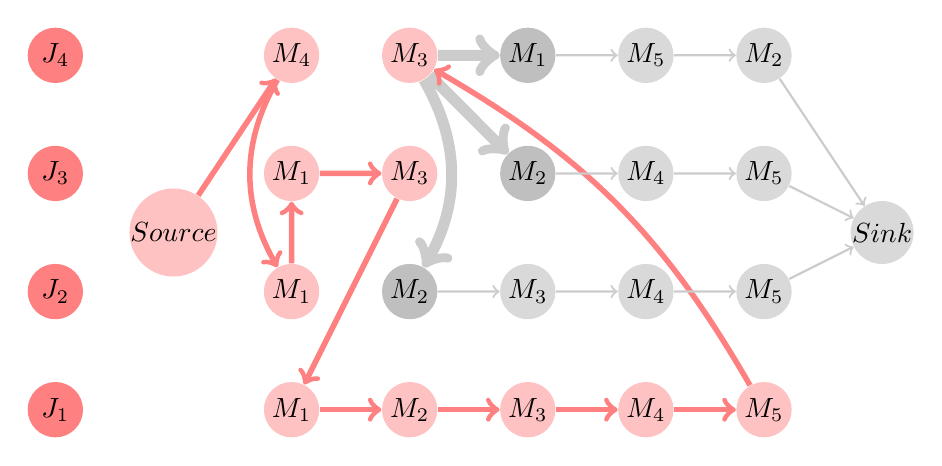
\begin{tikzpicture}[scale=1.5, auto, swap]
    % Draw the network
    % First we draw the jobs
    \foreach \pos/\name in {{(-1,0)/J_1},{(-1,1)/J_2},{(-1,2)/J_3},{(-1,3)/J_4}}
    \node[job vertex] (\name) at \pos {$\name$};    
    % Second draw the machines / vertices    
    \foreach \pos/\name/\mac/\proc in {{(6,1.5)/Sink},
        {(3,1)/J2M3/M_3/86},{(4,1)/J2M4/M_4/68},{(5,1)/J2M5/M_5/84},
        {(4,2)/J3M4/M_4/33},{(5,2)/J3M5/M_5/96},
        {(4,3)/J4M5/M_5/99},{(5,3)/J4M2/M_2/47}}
    \node[vertex] (\name) at \pos {$\mac$};
    \foreach \pos/\name/\mac/\proc in {{(0,1.5)/Source}, 
        {(1,0)/J1M1/M_1/26},{(2,0)/J1M2/M_2/25},{(3,0)/J1M3/M_3/40},{(4,0)/J1M4/M_4/15},{(5,0)/J1M5/M_5/42},
        {(1,1)/J2M1/M_1/18},
        {(1,2)/J3M1/M_1/20},{(2,2)/J3M3/M_3/23},
        {(1,3)/J4M4/M_4/13},{(2,3)/J4M3/M_3/55}}
    \node[completed vertex] (\name) at \pos {$\mac$};
    \foreach \pos/\name/\mac/\proc in {
    {(2,1)/J2M2/M_2/86},{(3,2)/J3M2/M_2/59},{(3,3)/J4M1/M_1/40}}
    \node[possible vertex] (\name) at \pos {$\mac$};
    % Selected trajectory
    \path[possible edge] (J4M3) to[bend left] (J2M2);
    \path[possible edge] (J4M3) to (J3M2);
    \path[possible edge] (J4M3) to (J4M1);
    \path[completed edge] (J4M4) to[bend right] (J2M1);
    \path[completed edge] (J1M5) to[bend right=15] (J4M3);
    \foreach \source/ \dest in {
        Source/J4M4, J2M1/J3M1, J3M1/J3M3, J3M3/J1M1, J1M1/J1M2, 
        J1M2/J1M3, J1M3/J1M4, J1M4/J1M5} 
    \path[completed edge] (\source) -- (\dest);
    % Connect vertices with edges 
    \foreach \source/ \dest in {
        J2M2/J2M3,J2M3/J2M4,J2M4/J2M5,J2M5/Sink,
        J3M2/J3M4,J3M4/J3M5,J3M5/Sink,
        J4M1/J4M5,J4M5/J4M2,J4M2/Sink}
    \path[edge] (\source) -- (\dest);
    \end{tikzpicture}
    }\\
    \subcaptionbox{$k=20$\label{fig:example:graph:final}}{
    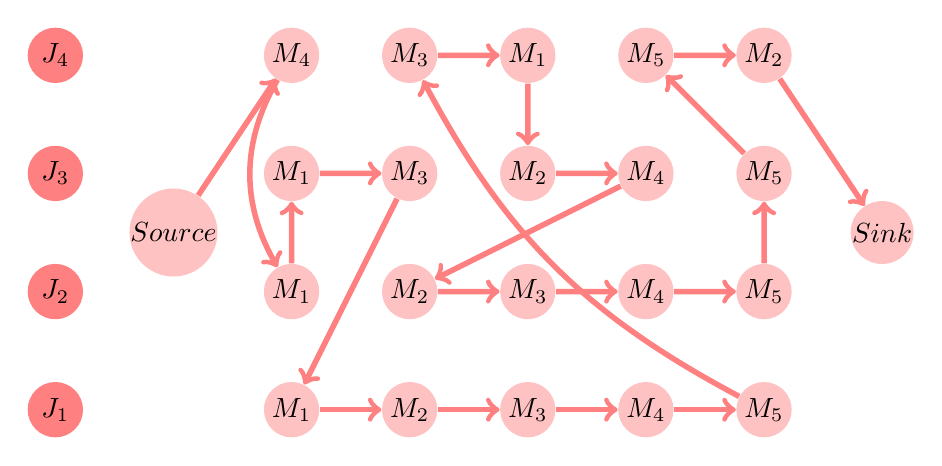
\begin{tikzpicture}[scale=1.5, auto, swap]
    % Draw the network
    % First we draw the jobs
    \foreach \pos/\name in {{(-1,0)/J_1},{(-1,1)/J_2},{(-1,2)/J_3},{(-1,3)/J_4}}
    \node[job vertex] (\name) at \pos {$\name$};    
    % Second draw the machines / vertices
    \foreach \pos/\name/\mac/\proc in {{(0,1.5)/Source},{(6,1.5)/Sink},
        {(1,0)/J1M1/M_1/26},{(2,0)/J1M2/M_2/25},{(3,0)/J1M3/M_3/40},{(4,0)/J1M4/M_4/15},{(5,0)/J1M5/M_5/42},
        {(1,1)/J2M1/M_1/18},{(2,1)/J2M2/M_2/86},{(3,1)/J2M3/M_3/86},{(4,1)/J2M4/M_4/68},{(5,1)/J2M5/M_5/84},
        {(1,2)/J3M1/M_1/20},{(2,2)/J3M3/M_3/23},{(3,2)/J3M2/M_2/59},{(4,2)/J3M4/M_4/33},{(5,2)/J3M5/M_5/96},
        {(1,3)/J4M4/M_4/13},{(2,3)/J4M3/M_3/55},{(3,3)/J4M1/M_1/40},{(4,3)/J4M5/M_5/99},{(5,3)/J4M2/M_2/47}}
    \node[completed vertex] (\name) at \pos {$\mac$};
    % Selected trajectory
    \path[completed edge] (J4M4) to[bend right] (J2M1);
    \path[completed edge] (J1M5) to[bend left=17] (J4M3);
    \foreach \source/ \dest in {
        Source/J4M4, J2M1/J3M1, J3M1/J3M3, J3M3/J1M1, J1M1/J1M2, J1M2/J1M3, 
        J1M3/J1M4, J1M4/J1M5, J4M3/J4M1, J4M1/J3M2, J3M2/J3M4, J3M4/J2M2, 
        J2M2/J2M3, J2M3/J2M4, J2M4/J2M5, J2M5/J3M5, J3M5/J4M5, J4M5/J4M2, 
        J4M2/Sink} 
    \path[completed edge] (\source) -- (\dest);
    \end{tikzpicture}
    }
    \caption[Graph representation for \jsp]{Graph representation of a 
    $4\times5$ \jsp, where pink vertices are completed tasks, and grey are 
    unassigned. Moreover, grey arrows point to the operations that are 
    next on the job-list, $\mathcal{L}^{(k+1)}$, and pink arrows 
    (traversing from source towards sink) yield the sequence of operations for 
    the schedule, i.e., $\vchi$.}\label{fig:example:graph}
\end{figure}
